\chapter{Introduction}

\section{Motivation}

From robots used for the automation of industrial processes to personal assistants robots and exploring robots for areas of difficult access, in the robotics area, we observe several applications with approaches from the least to the most complex in order to solve the most varied problems. Therefore, in order to develop the most distinct solutions, robotics appears as a multidisciplinary field, covering different lines of research, such as artificial intelligence, electronics, control algorithms, embedded systems, among many others.

One of the most prominent areas today is mobile robots, which aim to solve more complex tasks, in which the robot needs to move to carry out its activities. The difficulty of this branch is in how to control and coordinate the actions of robots so that they can interact with the environment and achieve their goal. For the accomplishment of some tasks, only one robot is not enough, being necessary then to use multiple robots, which makes the system more complex. Such systems prove how it is indispensable to have a control architecture for the coordination of all robots and a model of the organization of the system, capable of managing all the tasks that robots must perform, in order to achieve the system's objective, as can be seen in \cite{ACMultiplosRobos} and \cite{Moise}.

At the same time, in the line of development of control architectures for modeling intelligent agents in robotics, one of the fronts is the use of behavior trees to build the behavior of intelligent agents. Behavior trees were already widely used in the game development scenario, for modeling the behavior of non-player characters, and, thanks to their modularity and flexibility, they have been gaining more and more notoriety in robotics as a control architecture \cite{BTsInRobotics}.

Thus, it is possible to take advantage of the structure provided by the behavior trees to model systems in which it is necessary to control the actions of several robots, being able to model both the behavior of the robots with behavior trees, as well as the strategy that will coordinate all robots.

\section{Project Context}

\subsection{The ThundeRatz Robotics Team}

In order to develop national robotics and participate in academic competitions, the robotics team at the Polytechnic School of the University of São Paulo was founded in 2001. This team, initially called \textit{Los Cuervos}, was reformed in 2005, giving rise to ThundeRatz \cite{ThundeRatz}.

Currently supervised by Prof. Dr. Rafael Traldi Moura, the group aims to learn about several topics that touch the state of the art of robotic systems, having contact with the newest lines of research. All this technical knowledge is used to design projects that encompass several areas of engineering, so that the team can submit these projects to test in national and international robotics competitions, gaining prominence on the robotics world stage.

At the moment, the team has several projects, having combat robots, sumo, hockey robots and autonomous robots that perform the most varied tasks, such as playing soccer or following a line on the ground.

\begin{figure}[!h]
    \centering
    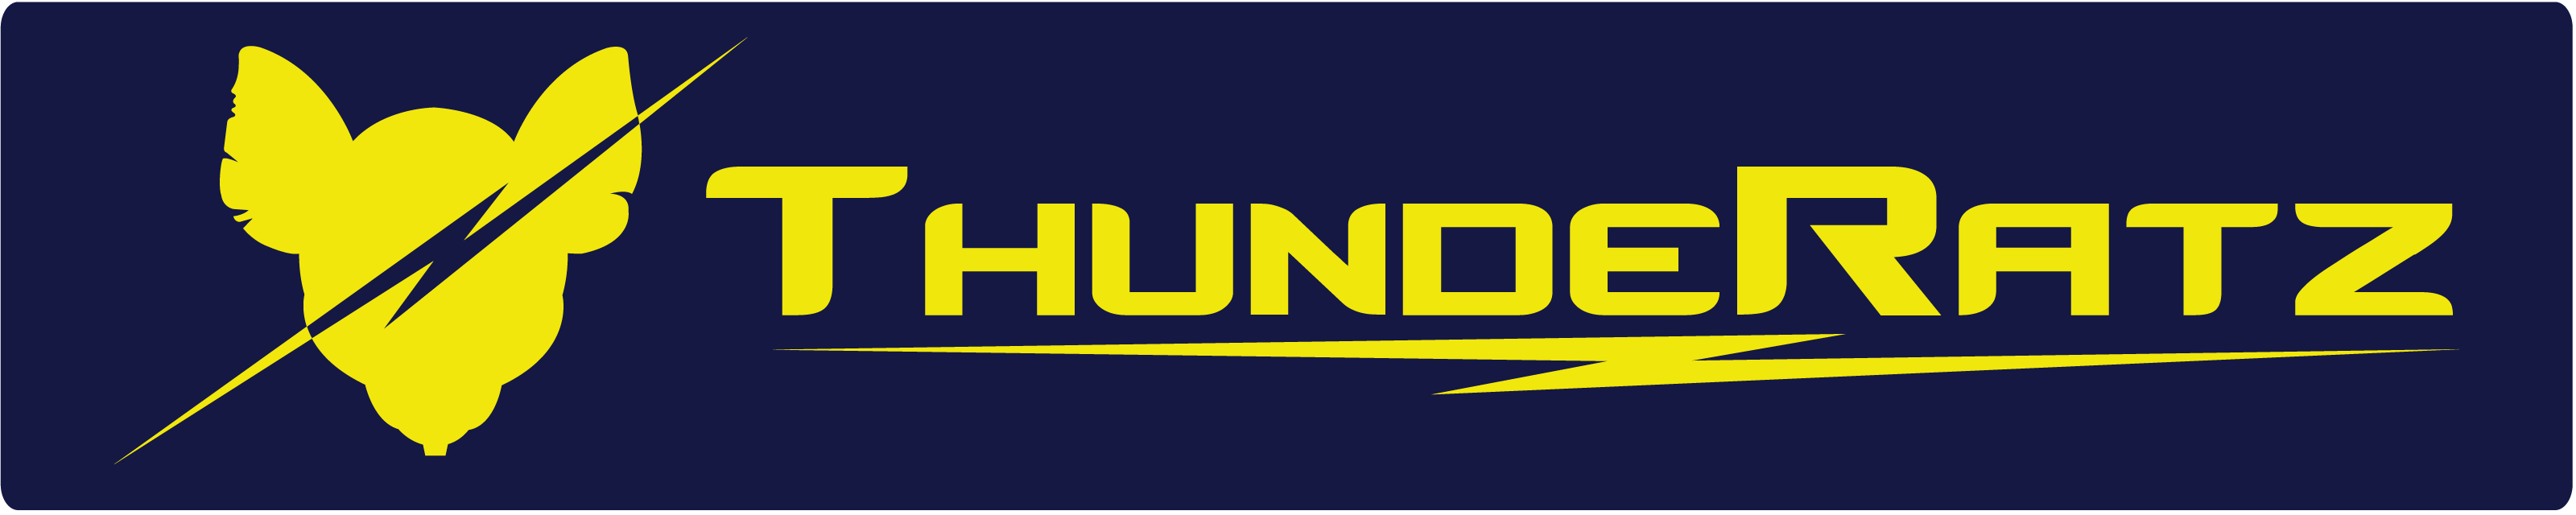
\includegraphics[width=.6\linewidth]{chapters/introduction/images/ThundeRatz Logo.png}
    \caption{ThundeRatz's logo. Taken from \cite{ThundeRatz}}
\end{figure}

\subsection{The IEEE Very Small Size Soccer (VSSS) category}

One of the most challenging and stimulating academic robotics competition categories is the \textit{IEEE Very Small Size Soccer (VSSS)} category. In this category, competitors must develop an engineering solution for a team of robots that must play soccer autonomously, being each team composed of three players, each with maximum dimensions of 75 mm x 75 mm x 75 mm. The match is played on a 130mm x 150mm field and consists of two game periods, each lasting five minutes, with a half-time break of ten minutes.

Originally, the category had only its version with physical robots, in which matches are played on a black field with white markings and the robots have colored markings on their top, so they can be identified by means of a camera located above the field. However, due to the COVID-19 pandemic, the category adapted to the health context and also started to occur in a simulated environment, using the FIRASim \cite{FIRASim} simulator.

For the physical version, in addition to game strategies, the teams need to develop the mechanical and electronic system of the robots, as well as a computer vision system to identify the positions and speeds of the robots in the field and a communication system between the computer that runs game strategy and physical robots, for the transmission of movement commands.

As for the simulated version, there is no need to develop the parts of the systems related to the physical world, only the system to determine the game strategy and a communication interface with the game simulator and with an automatic judge \cite{VSSReferee} developed for the category.

\begin{figure}[!h]
    \centering
    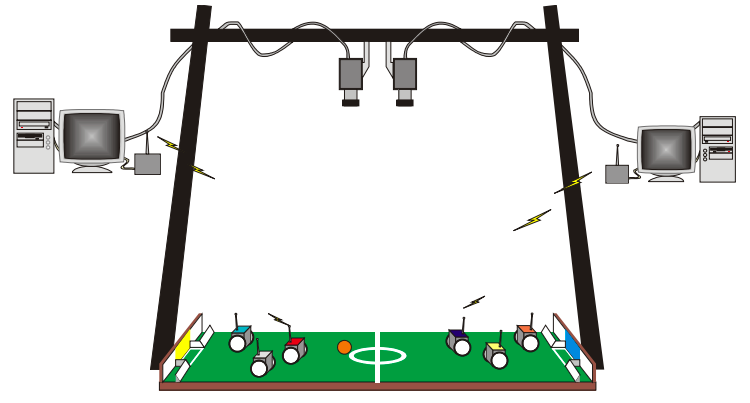
\includegraphics[width=.7\linewidth]{chapters/introduction/images/General System.png}
    \caption{Representative scheme of the system used in the category. Taken from \cite{FutRobosFerramentaDeEnsino}}
    \label{fig:general_system}
\end{figure}

\subsection{The ThunderVolt Team}

To participate in the \textit{VSSS} category, the ThundeRatz team developed a team of robots called ThunderVolt \cite{ThunderVolt, TDPThunderVolt}.

For its physical version, four robots were developed, called: Alan, Dorothy, Grace and Alex. Each one was inspired by a figure in science and engineering, with the honorees being, respectively, Alan Turing, Dorothy Vaughan, Grace Hopper, and Alessandro Volta. In addition, a computer vision system was developed, using the library \textit{OpenCV} \cite{OpenCV}, as well as a communication system with the physical robots, by the means of using the radio frequency modules nRF24L01 alongside an open source library developed by team \cite{STM3232RF24}. Meanwhile, for its simulated version, a communication interface with the simulator and the automatic judge was developed using the UDP protocol.

\begin{figure}[!ht]
    \centering
    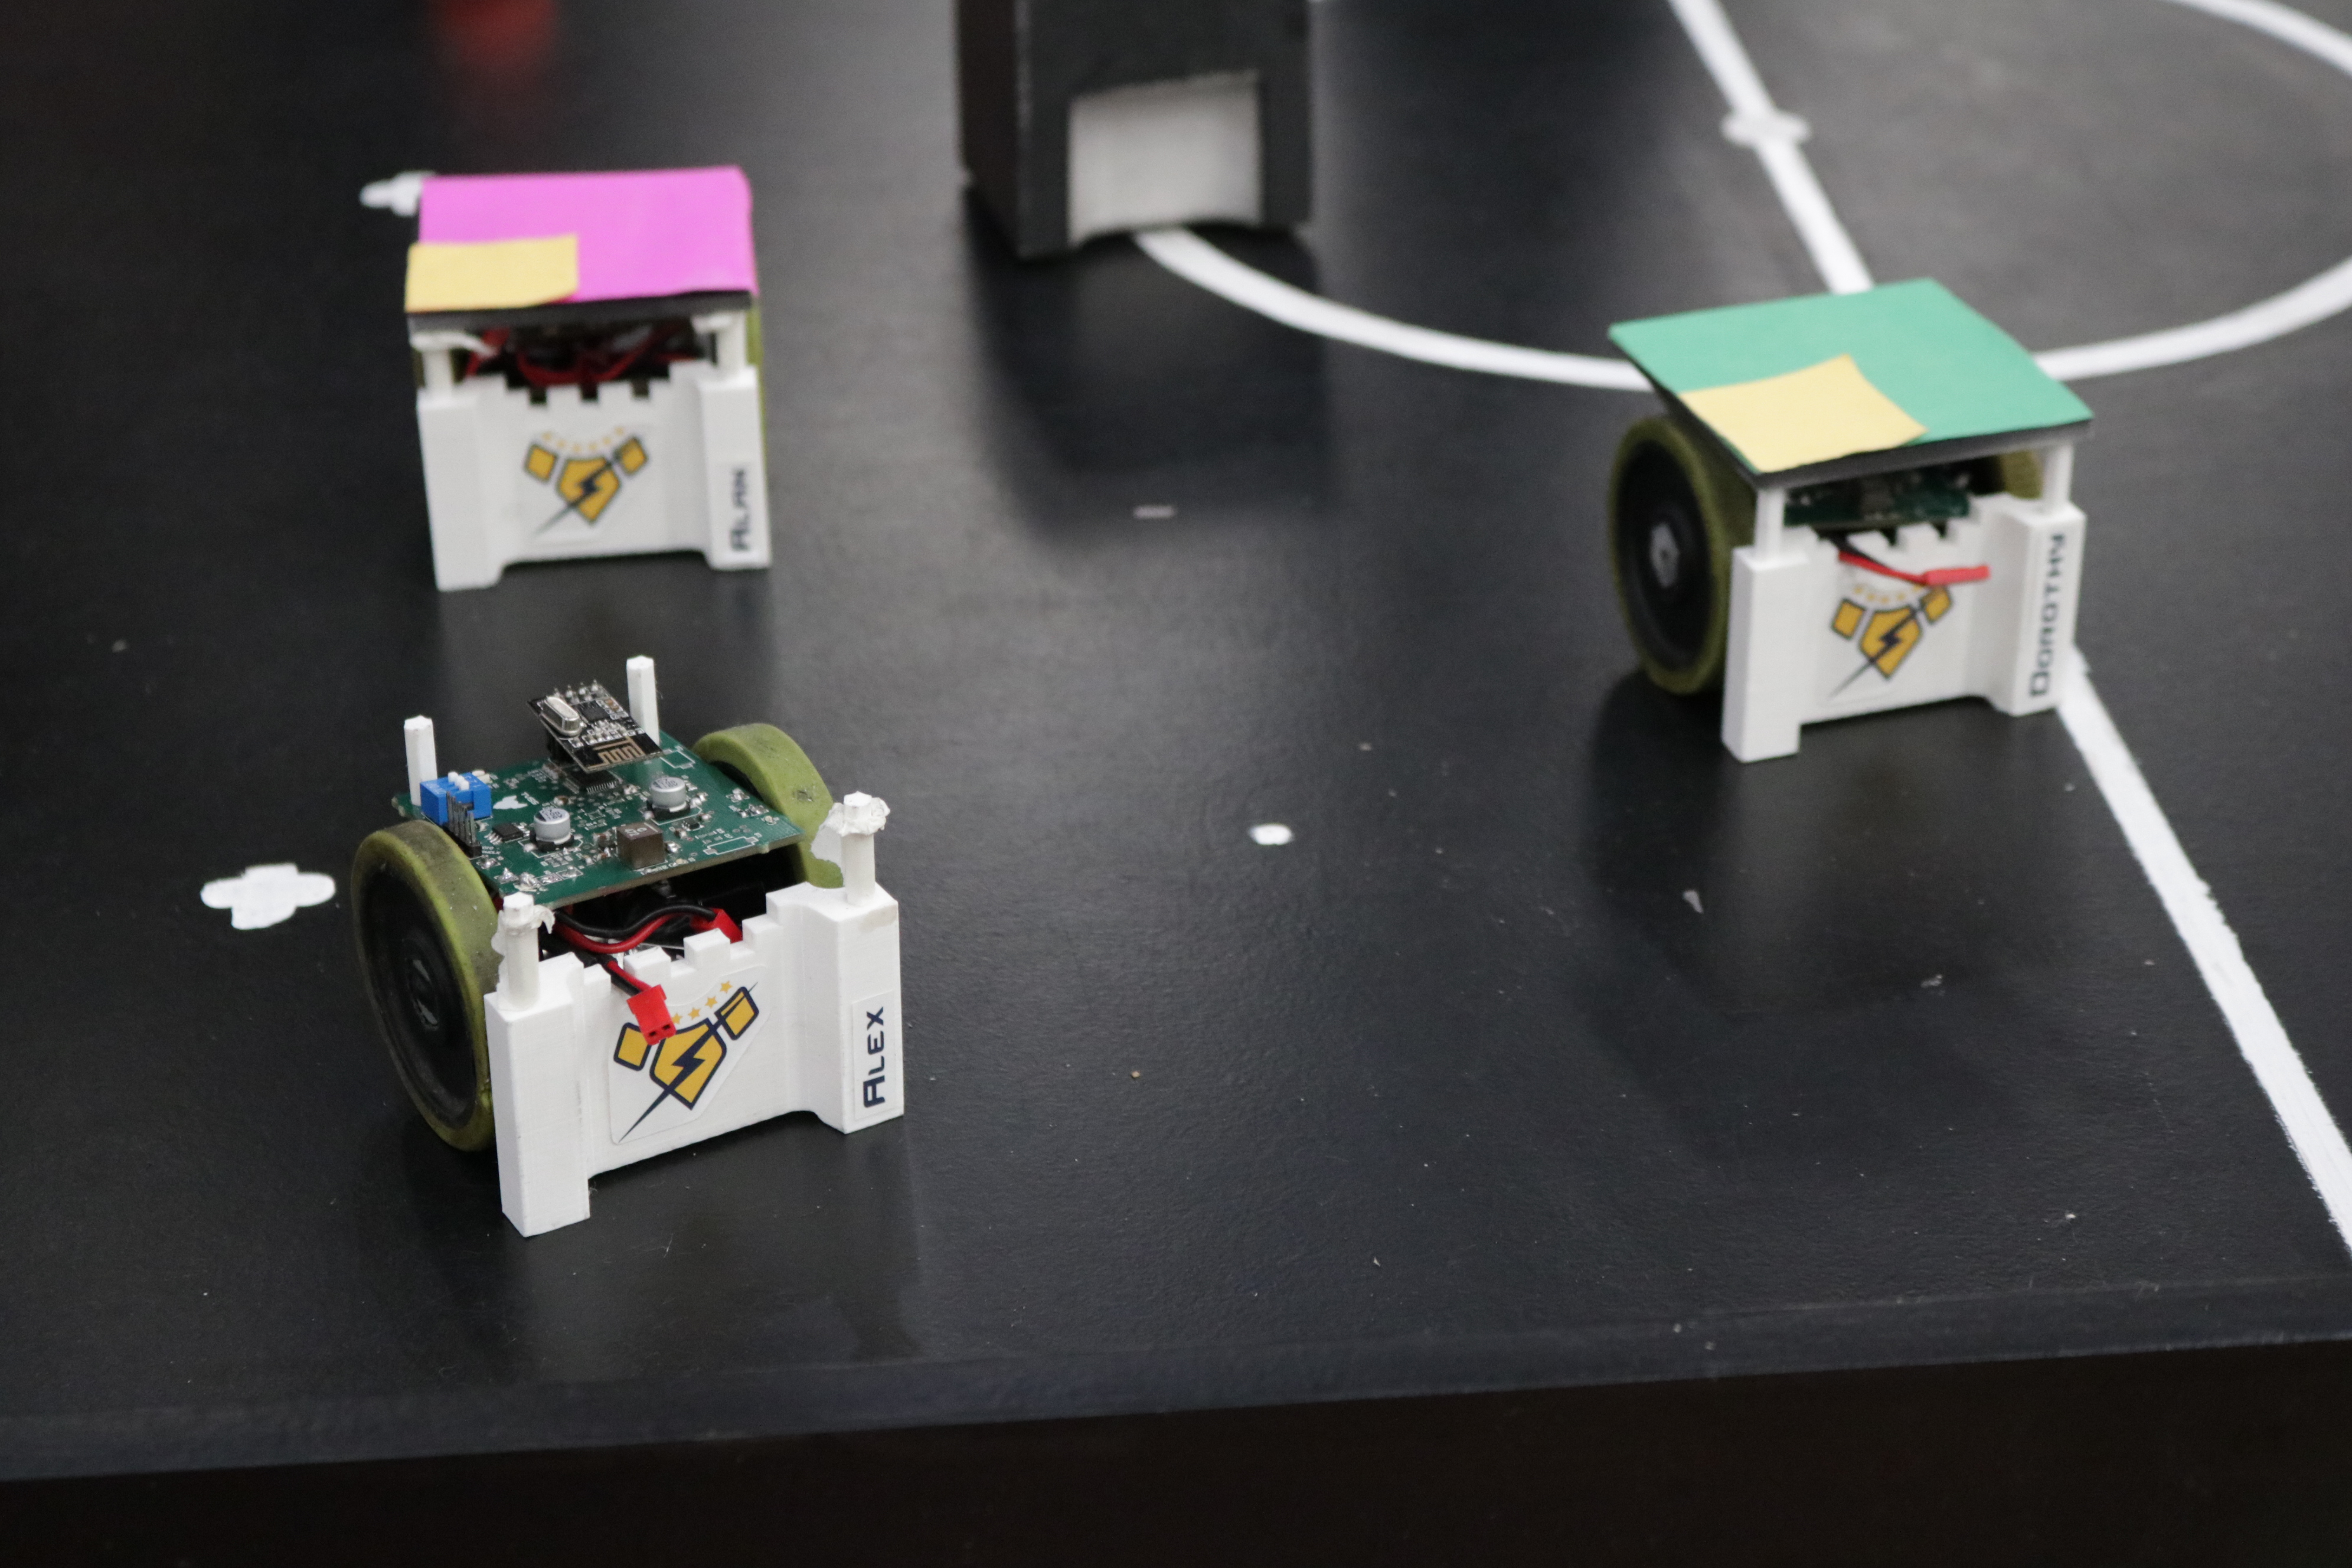
\includegraphics[width=.6\linewidth]{chapters/introduction/images/ThunderVolt Robots.jpeg}
    \caption{ThunderVolt team physical robots. Taken from \cite{ThunderVolt}}
    \label{fig:physical_robots}
\end{figure}

Regarding the central system that determines the strategy of the game and controls the robots, its architecture was implemented based on the \textit{Robotic Operating System (ROS)} \cite{ROS}, a framework that provides several tools and libraries useful for developing robotics applications. This central system was divided into two main parts, the specification of different roles that a robot can play and a Coach entity. 

The specification of the roles consists of previously implemented behavior trees, which use the information of the current state of the game, navigation methods, like vector fields-based navigation \cite{VectorFields}, and control algorithms, like PID controllers, to determine what a robot should do in a specific state of the game and how it should do it. 

On the other hand, the Coach entity is the one responsible for coordinating the robots, that is, controlling whether they should play or not and which role each robot should play. In the initial implementation, a Finite State Machine (FSM) was employed to model this coordination system. However, as the project progressed, it became evident that the FSM approach did not scale effectively. The system grew increasingly complex, making it challenging to comprehend, maintain, and implement improvements. Therefore, it was necessary for the project to seek better solutions for the control architecture of the coordination system.

\section{Objectives}

This work aims to improve the architecture, maintainability, flexibility to changes, and, if possible, the performance of the ThunderVolt team, in the competitions of the \textit{VSSS} category of autonomous robot soccer. In order to achieve that, the goal of this work is to introduce a new cooperation strategy based on an organizational model \cite{Moise} of agents, using behavior trees to model how the roles assignments should be performed in the organization. Thus, the objective of this work will involve the central system for determining the team's strategy, without impacting the other systems used in the project.

\section{Justification}

Extensive research has been conducted in the field of control architecture in robotics, presenting and comparing the use of different control architectures for the implementation of the most varied use cases \cite{BTsInRobotics, SurveyBTs, Expressiveness, iovino2022programming, RobotArchitectureInDynamicEnvironment, PetriNetsRobotics, billington2010plausible, BTsAndFSMApplications}. 

Among these architectures, Finite State Machines (FSMs) and Hierarchical Finite State Machines (HFSMs) have always had great dominance in robotics applications, since they are very well established and mature architectures. However, it is important to highlight how the use of Behavior Trees (BTs) has grown a lot in recent years, becoming a very popular control architecture and almost as used as FSMs and HFSMs. This fact can be observed in \cite{BTsAndFSMApplications}, in which a survey of the number of applications utilizing different libraries to implement robot behavior using the mentioned control architectures was performed.

Besides the fact that they are very mature control architectures, the wide use of FSMs and HFSMs can also be justified by the fact that they are very easy to understand and implement, facilitating the development of applications \cite{BTsInRobotics, Expressiveness, iovino2022programming}. Nonetheless, as presented in \cite{BTsInRobotics, SurveyBTs, iovino2022programming}, when implementing more complex applications, it is possible to notice how FSMs grow fragile, not scaling well with the size of the application and becoming very difficult to understand.

In contrast, BTs are very expressive, modular, and flexible structures. In \cite{BTsInRobotics}, it is shown how BTs can generalize many other control architectures, such as the Subsumption Architecture, the Teleo-Reactive Paradigm, Decision Trees, and even FSMs \cite{BTsInRobotics, Expressiveness,  iovino2022programming}. Regarding expressiveness, the most similar control architecture to the BTs is the HFSMs, which is a very powerful robust architecture, presenting, however, the already mentioned drawbacks. Therefore, the BTs present themselves as a great control architecture to be used to improve the control strategy of the ThunderVolt team, so it can become more scalable, modular, and easier to maintain.

Furthermore, it is worth noting that in the majority of the presented research studies, the focus is more on the implementation of individual agent behaviors and the comparison of different control architectures. There are other papers that focus on coordinating multi-agent systems, such as the article \cite{Event-DrivenBTs}, which is more focused on game applications, and other advances in the field of robotics, such as \cite{Self-ReactivePlanningOfMulti-Robots, BTsMultRobot}. 

In \cite{Event-DrivenBTs}, an extension of BTs to address the coordination of non-player characters is proposed, presenting a way of developing an agent that can react to events and can communicate with other agents. On the other hand, \cite{Self-ReactivePlanningOfMulti-Robots} introduces a method of coordinating swarms of robots using a BT that formalizes a coordination behavior and applying this BT to all robots, so that the robots can exchange information with each other to perform a task. However, in this article, it is not described how to handle the part of assigning tasks to robots with a BT. In \cite{BTsMultRobot}, the advantages of using BTs in multi-robot systems are presented, showing BTs that can be used to perform specific tasks and others to handle the assignment of tasks to agents in the system, but not handling task switches between the robots. 

Thus, the ThunderVolt project is an excellent case study for the use of BTs in multi-agent organizations, extending the research of the presented works, as the project needs to constantly react to changes in real-time, not just when events are received, and needs to dynamically assign tasks to the robots and switch tasks between the robots, by the means of using a BT.

\section{Project Organization}

This work is divided into eight chapters, with this introduction being the first.

In Chapter \ref{ch:background}, a review of the literature is performed, covering the key theoretical foundations necessary to comprehend this project.

In Chapter \ref{ch:methodology}, the methodologies employed throughout the project will be outlined, providing insights into how the work was executed.

In Chapter \ref{ch:target_system}, the relevant information of the target system of this work, the ThunderVolt team, will be explained, detailing the rules that the project needs to follow and how it worked prior to the proposed changes, describing its previous structure and the old game strategy.

In Chapter \ref{ch:requirements}, the requirements of the team improvement proposal will be described, defining functional and non-functional requirements.

In Chapter \ref{ch:development}, a deep explanation of the new strategy specification and implementation will be performed, highlighting the technologies used in the process.

In Chapter \ref{ch:results}, the results of utilizing the new strategy will be presented and discussed. Additionally, a comparative analysis between the old and the new strategy will be performed.

Finally, in Chapter \ref{ch:final_considerations}, the final considerations of the project will be elucidated and the contributions of this work will be described.
